\documentclass[12pt]{report}

%% Language and font encodings
\usepackage[english]{babel}
\usepackage[utf8]{inputenc}
\usepackage[T1]{fontenc}
\usepackage{lscape}
%\usepackage{subfigure}
%% Sets page size and margins
\usepackage[a4paper,top=3cm,bottom=3cm,left=3cm,right=3.5cm,marginparwidth=1.75cm]{geometry}
\usepackage{fancyhdr}
\renewcommand{\baselinestretch}{1.5}

\newcommand{\HRule}{\rule{\linewidth}{0.5mm}}
\newcommand\frontmatter{%
    \cleardoublepage
  %\@mainmatterfalse
  \pagenumbering{roman}}

\newcommand\mainmatter{%
    \cleardoublepage
 % \@mainmattertrue
  \pagenumbering{arabic}}


\pagestyle{fancy}
%%

%% create an alias for \mathbf{}
\newcommand{\myvec}[1]{\mathbf{#1}}

\usepackage{gensymb}
\usepackage{mathtools}
\usepackage{todonotes}
\usepackage{biblatex}
\usepackage{graphicx}
\usepackage{caption}
\usepackage[justification=centering]{subcaption}
\addbibresource{references.bib}

\begin{document}

\begin{titlepage}
\begin{center}
\textsc{\LARGE Università di Pisa}\\ % University name
Dipartimento di Ingegneria dell'Informazione\\
Corso di Laurea Specialistica in Computer Engineering\\[1cm]
\begin{figure}[h]
\centering
\includegraphics[scale=0.5]{img/Unipi_logo}
\end{figure}

\textsc{\Large Laurea Specialistica in Computer Engineering}\\[0.5cm] % Thesis type

\HRule \\[0.4cm]
{\huge \bfseries 3D Environments Reconstruction using 360 Videos}\\[0.1cm] % Thesis title
\HRule \\[1cm]
 
\begin{flushleft} \large
\emph{Supervisors:}\\
Marco AVVENUTI\\
Francesco BANTERLE \\
Massimiliano CORSINI% Supervisor name - remove the \href bracket to remove the link  
\end{flushleft}

\begin{flushright} \large
\emph{Candidate:}\\
Andrea BECONCINI\\[1.5cm] % Author name - remove the \href bracket to remove the link
\end{flushright}
 
% \large \textit{A thesis submitted in fulfilment of the requirements\\ for the degree of \degreename}\\[0.3cm] % University requirement text
% \textit{in the}\\[0.4cm]
% \groupname\\\deptname\\[2cm] % Research group name and department name
 
{\large Academic Year 2016-17}\\[4cm] % Date
%\includegraphics{Logo} % University/department logo - uncomment to place it
 
\vfill
\end{center}

\end{titlepage}

\fancyhead[L]{\slshape \leftmark}
\fancyhead[R]{}

\frontmatter


\fancyhead[L]{\slshape \leftmark}
\fancyhead[R]{}

\frontmatter
\begin{abstract}
\thispagestyle{plain}
\addcontentsline{toc}{chapter}{Abstract}
360\degree degrees or full spherical images are gaining a huge interest in different fields such as autonomous driving, cinematography, augmented reality (AR), and virtual reality (VR).

Computer vision research addressing spherical images is less popular than the one that considers traditional perspective cameras. This new kind of devices have some advantages with respect to standard cameras, for example, it allows users to capture an entire environment in a single shot.

In this work, we developed a structure from motion (SfM) pipeline for full spherical cameras composed of two main parts: camera poses estimation and dense point cloud reconstruction. This pipeline employs frames captured using a 360\degree video-camera in the equirectangular format.

Our contribution includes: a visual-based frame filter that selects frames to be used for motion estimation, a novel SfM pipeline implementation in MATLAB, and an adaptive window matching 
procedure for point cloud densification.

We tested the performance of our work both with synthetic 3D scenes and with real sequences captured with a Ricoh Theta S camera.
\end{abstract}


\setcounter{page}{2}
\pagestyle{fancy} % The page style headers have been "empty" all this time, now use the "fancy" headers as defined before to bring them back
\addcontentsline{toc}{chapter}{Contents}
\lhead{\emph{Contents}} % Set the left side page header to "Contents"
\tableofcontents % Write out the Table of Contents
\cleardoublepage

\mainmatter
\chapter{Introduction}
The growing interest of general public in those technology that were 
research-only exclusives once, makes them cheaper and spread further and
animates research again.

The omnidirectional and full spherical cameras are some perfect examples for 
this trend.
These devices has been used in robotics since their first appearance and they 
can be exploited in today consumer technologies like Augmented and Virtual 
Reality devices and autonomous driving vehicles.

\section{Omnidirectional and Full Spherical Cameras}
\label{sec:cameraclassification}
Omnidirectional cameras are characterized by wide field of view (FOV), 
indeed many of this kind
of devices can take pictures with a 180\degree view angle or even wider.

There are several ways to obtain panoramic images that is by using:
\begin{itemize}
	\item perspective cameras and image stitching;
	\item catadioptric cameras;
	\item dioptric cameras;
	\item hybrid approaches.
\end{itemize}

Perspective cameras can take panoramic pictures with the aid of 
software stitching: first, we take several pictures with many cameras or by
simply moving 
the same camera in order to cover a larger scene. Then the stitching software 
creates a single picture out of the set of images.
The single perspective camera and the stitching software is the cheapest 
way to obtain panoramic images because it does not need any kind of specialized 
hardware. However it is impossible to record videos since the shooting phase 
requires time.

Catadioprict cameras are obtained with a perspective camera plus a mirror. 
The camera take a picture of the mirror which reflects the image of the 
surroundings. The mirror used to create a catadioptric system is shaped like a 


A traditional camera can also be adapted to work as a panoramic one by adding
fisheye lenses capable of refracting lights from wide angle towards the 
image sensor. This setup are called dioptric cameras.

Even though the devices described before 

\chapter{State of the Art}
\lhead{\chaptername~\thechapter. \emph{State of the Art}}
\label{ch:state_of_the_art}
%
In this chapter, we define formally the VO problem, we describe a generic perspective SfM pipeline, 
and then we introduce the main challenges and issues when employing full spherical cameras for VO.
During this description we refer, time by time, to the related state of the art algorithms/methods.

%
% Start of sections from intro

\section{SfM, VO, and SLAM}
SfM is a long studied topic in computer vision. Starting from an input of photographs taken by one or multiple cameras, SfM's main goal is to compute the cameras' poses and to reconstruct the 3D environment captured by those cameras.
%
Some of the first works are the paper by Longuet-Higgins\cite{longuet1981computer}, whose equations are fundamental in epipolar geometry, and the paper by Tomasi et al.\cite{tomasi1992shape}, who used orthographic photographs to estimate the shape of a 3D object.
%
SfM is a general term, and it also includes \textit{visual odometry} (VO). This is the problem of recovering the motion of an agent equipped with a camera rig in a 3D environment. Typically, VO deals with an ordered set of images such as video sequences, and it uses them to compute the egomotion in real-time. Nister et al.\cite{nister2004visual} introduced the term \textit{visual odometry} for the first time.

Another field of robotic/computer vision research that is very close to VO is \textit{simultaneous localization and mapping} (SLAM). SLAM targets the problem of creating a map of the environment where a camera equipped agent navigates and simultaneously estimating its path. Scaramuzza\cite{scaramuzzaVisualOdometryI} pointed out that while VO is more focused on local motion estimation, SLAM's goal is to obtain a global consistent estimation of the agent movements.
%
In order to reduce error, SLAM keeps track of the visited path and can decide when the agent has come back to a previously visited location. This extra step in SLAM's pipeline is called \textit{loop closure} and provides an additional constraint used to reduce errors in both the agent's path and 
environment reconstruction. Durrant-White et al.\cite{durrant1996localization} firstly introduced the term SLAM.
 
\section{Densification: from Sparse to Dense Point Cloud}
A sparse point cloud is the product of most SfM pipelines; some keypoints are tracked in each photograph and are then used by the motion estimation algorithm. These keypoints are triangulated and their corresponding world points are available during egomotion estimation.
%
A set of triangulated keypoints is a sparse point cloud around the camera's path. This set provides a first approximation of the environment reconstruction.
Typically, starting from this information, it is possible to obtain a complete reconstruction of the 3D environment by applying
a so-called \emph{Multi View Stereo} algorithm. The goal of Multi View Stereo\cite{seitz2006comparison} is to reconstruct a complete
3D object model from a collection of images taken from known camera poses.
Many of these algorithms obtain a dense point cloud starting from the sparse reconstruction, and then 
estimate the final surface according to this dense point set.

Our approach consists in densify the point cloud by computing, for each pair of consecutive images, 
a depth map. These depth maps are merged to obtain a dense set of reconstructed points. At this point the 
surface can be reconstructed by applying a surface fitting algorithm such as the standard Poisson reconstruction??CITARE??. 
A depth map consists in associating a value of depth for each pixels of the images pair.
The depth map estimation involves the calculation of a \textit{disparity map} from the images pair. 
This is a map of the distance in pixels from a point in a reference image and its corresponding point in the 
other image. Higher is the disparity of a given pixel, higher is the parallax and hence the depth of that pixel. 
The map is usually computed based on some kind of similarity 
metric such as \textit{sum of absolute distances} (SAD), 
\textit{sum of squared distances} (SSD), 
\textit{normalized cross correlation} (NCC), etc. These provides a way to 
compute the corresponding point in the second image, thus enabling the 
computation of the disparity for every point in the reference image.
Figure~\ref{fig:disparity_example} shows an example of disparity map.

\begin{figure}[h]
	\centering
	\begin{subfigure}{0.4\textwidth}
		\centering
		\includegraphics[width=0.7\textwidth]{img/aloe_view1}
	\end{subfigure}
	\begin{subfigure}{0.4\textwidth}
		\centering
		\includegraphics[width=0.7\textwidth]{img/aloe_disparity}
	\end{subfigure}
	\caption{\label{fig:disparity_example}An example of disparity map from the
	Middlebury dataset \cite{hirschmuller2007evaluation}}
\end{figure}

\section{Omnidirectional and Full Spherical Cameras}
\label{sec:cameraclassification}
Omnidirectional cameras are characterized by wide field of view. Indeed, many of this kind of devices can take pictures with a 180\degree view angle or even wider.

There are several ways to obtain panoramic images, they include:
\begin{itemize}
	\item perspective cameras and image stitching;
	\item catadioptric cameras;
	\item dioptric cameras;
	\item hybrid approaches.
\end{itemize}

Perspective cameras can take panoramic pictures with the aid of software stitching. As the first step, we take several photographs with many cameras or by simply moving the same camera in order to cover most of a scene. Then, a stitching software merges all images into a single one. To use a traditional camera and a stitching software is the cheapest way to obtain panoramic images because it does not need any kind of specialized hardware. However, this process is cumbersome (a lot of manual work is required). Note that some smart-phones provide built-in camera 360\degree acquisition modes, but the final quality may be not satisfactory due to alignment artifacts.
An example for this approach is the Hugin Panorama Photo Stitcher 
\cite{hugin_photostitcher}, an open source software for merging several 
perspective images in a single panoramic picture.
The SpheroCam\texttrademark by SPHERON-VR AG\texttrademark \cite{spheronvr}
is an alternative to 
the latter approach to panoramic images; it uses a specialized hardware composed
of a wide angle lenses equipped camera mounted on a rotating support, which rotates around the optical center of the camera. Therefore, this camera can capture high quality full spherical and it addresses the professional fields of geographical analysis, forensic investigation, cultural heritage, etc.

A catadioptric camera can be obtained by coupling a perspective camera and a mirror, which is mounted in front of camera. Such setup takes a picture of the mirror that reflects the surrounding. The mirror of a catadioptric system may have several shapes. The most common one is the hyperbolic profile that creates a single center of projection for every ray coming to the mirror.

A traditional camera can also be adapted to work as a panoramic one by adding a fisheye lens capable of refracting lights from wide angle towards the image sensor. These setups are called dioptric cameras.

Apart of perspective cameras coupled with stitching software, none of the previous approaches can take full spherical panoramic photographs. Moreover, full spherical videos cannot be shot with perspective cameras either.

The last approach, an hybrid one, exploits several sensors using fisheye lenses and software stitching to capture full spherical panoramic images in a single shot. This enables full spherical video capturing as well. The camera (that is composed of several image sensors) take multiple overlapping pictures simultaneously. Then, an on camera stitching software composes the data in a single image.

In all our experiments we used the Ricoh Theta S\registered camera that is a hybrid full spherical camera composed of two fisheye lenses with a FOV greater than 180\degree; see Figure~\ref{fig:ricoh_theta}.
%
%
% end of sections from intro

\section{VO Problem}
\label{sec:vo_problem}
As we described in the previous chapter, the VO's goal is to recover the 
camera trajectory while it is moving in the environment. Following Scaramuzza and Fraundorfer\cite{scaramuzzaVisualOdometryI},
we introduce the notations that we are going to use for the rest of this work.
%
Let first assume time is sampled in a sequence of time instants \(k\); 
\(I_{0:(n - 1)} \) is the set of $n$ input frames, where \(I_{k}\) is a picture taken by 
the camera at time \(k\). We define \(C_{0:(n-1)}\) as the set of camera 
positions such that \(C_k\) is the position at the \(k\)-th time.
If we call \(T_k\) the rigid body transformation of the camera between two
consecutive time instants (i.e., $k-1$ and $k$), then we have the following relation:
%
\begin{equation}
	C_k = C_{k-1} T_k
	\label{eq:motion_composition}
\end{equation}
%
\noindent where \(T_k\) is defined as
%
\begin{equation*}
	T_k =
	\begin{bmatrix}
	R_k & \myvec{t}_k \\
	0 & 1
	\end{bmatrix} \text{,}
\end{equation*}
%
\noindent where $R_k$ is a 3-by-3 rotation matrix (i.e., the rotation of the camera at time $k$),
$\myvec{t}_k$ is a column vector (i.e., translation of the camera at time $k$).
Therefore, the goal of VO is to estimate both $R_k$ and $t_k$ for each time 
$k$ and to compute each $C_k$ accordingly to equation~\ref{eq:motion_composition}. Note that the initial position $C_0$ can be set arbitrarily.

Equation~\ref{eq:motion_composition} is the core of VO, that allows us to compute the camera local movement. Therefore, we can estimate its location in every instant of time. However, the equation above contains also the most insidious practical challenge of VO; i.e., the error accumulation phenomenon known as \textit{drift}.
Every new position $C_k$ can introduce an error factor that affects the next 
computations. The results is a global error that grows as the number of 
estimations increases.
%
Since early works such as Harris et al.\cite{harris19883d} and Moravec\cite{moravec1980obstacle}, the VO research community has focused on error minimization techniques to reduce drift.
This tackles the precise estimation problem either by employing more accurate
local motion estimation and by introducing an optimization step to refine 
camera locations.
The set of techniques for reducing the drift (after the camera poses are computed) is typically called  \textit{bundle adjustment}.

\section{Perspective SfM}
The SfM literature is vast, but most of the approaches present pipelines similar to the one in 
Fig.~\ref{fig:block_diagram}.
The main steps are: to compute the relative motion for each image
pair, to compose these motions for obtaining the absolute camera position and 
orientation, and to run a drift reduction procedure.
%
The differences are in the type of input data, motion estimation algorithm,
optimization procedure and additional constraints considered.
For generic SfM researches, the input data is a set of traditional pictures of 
the same environment from different point of view. The pictures can be taken by 
different cameras with unknown parameters and in different time instants.
%
\begin{figure}
	\centering
	\def\svgwidth{0.5\columnwidth}
	\input{img/block_diagram.pdf_tex}
	\caption{Perspective SfM pipeline block diagram.}
	\label{fig:block_diagram}
\end{figure}

\textit{Visual Odometry} is based on SfM techniques, 
in this case, the input data is usually a sequence 
of images from a video stream. The image capturing devices can vary:
Moravec used a sliding camera that could capture stereo images \cite{moravec1980obstacle} while Matthies et al. equipped their robot with
an actual stereo rig \cite{matthies1987error};
in \cite{nister2004visual} Nister et al used a single perspective camera.
The computer vision literature refers to the
single camera studies case with the term \textit{monocular VO} while it uses \textit{stereo VO} to describe the work done with stereo equipment.

Even though perspective cameras have been the first choice in many studies, 
the researchers used other devices, like the ones described in 
\ref{sec:cameraclassification}.

We use the terms \textit{perspective} or \textit{traditional SfM} to describe 
SfM pipelines designed for perspective cameras.

A great resource about the state of the art for VO and SfM is the work by Scaramuzza and Fraundorfer,  
\cite{scaramuzzaVisualOdometryI, scaramuzzaVisualOdometryII}.

\subsection{Motion Estimation}
\label{subsec:motion_estimation}
We use the term local motion to indicate the camera movement between two 
consecutive images while, on the other hand, we define global motion as
the overall camera's path.
The local motion estimation step is fundamental in a SfM pipeline, its goal is 
to find the rigid body transformation composed of $R_k$ and $t_k$ as we 
described in Section~\ref{sec:vo_problem}.
All the local motion estimation methods described in the literature so far are 
based on the correspondences found in two consecutive images but, depending on the
specific camera rig (stereo imaging systems or monocular), the type of 
correspondences and their matching procedure, we may have several choices for
the actual way to estimate local motion.
There are two main families of point matching algorithms: \textit{feature-based}
and \textit{appearance-based} (also known as \textit{global-methods}).
While the former ones utilize repeatable features 
matching between the images, the latter rely on pixel's intensity information; 
they are simpler but also slower. Most of the 
most recent VO pipelines use feature-based methods because of
their speed and robustness.
A VO implementation that employs intensity based techniques is 
\cite{nister2004visual}, while \cite{makadia2007correspondence} is an example 
of featureless motion estimation method.

Each of the feature points found by the motion estimation phase can be 
either a 3D world-point feature or a 2D image-point one,
therefore, there are three possible combinations that provides just as many 
different matching and motion-estimation procedures:
\begin{itemize}
	\item 2D-to-2D: both feature sets are composed of image points.
The matching metric can be a simple euclidean distance between feature 
descriptors and the motion estimation can be solved by estimating the 
\textit{essential matrix} (see section~\ref{subsec:essential_matrix} for 
details);
	\item 3D-to-3D: both feature sets contain world-points features and motion
estimation is performed by solving an alignment problem;
	\item 3D-to-2D: the previous image's feature set is composed of world points while
the current one's feature set contains their projections. In this case, the motion 
is estimated by solving a problem called Perspective-n-Points (\textit{PnP}).
\end{itemize}
Since the second and third approaches deal with 3D points, they are usually 
best suited for stereo rig (especially the 3D-to-3D case).
Obviously, we can still use the 3D-to-2D approach in the monocular VO case by simply 
triangulating corresponding 2D image features in consecutive frames.
In fact, in order to obtain the first 3D feature set,
we can compute the relative motion between the first two images with 
the 2D-to-2D techniques and then obtain the rest of the camera's path,
as we said, by solving the \textit{PnP} problem.

\subsubsection{Essential Matrix}
\label{subsec:essential_matrix}
The essential matrix $E$ is defined as
%
\begin{equation}
\label{eq:epipolar_equation}
	\myvec{p}^{\prime\top} E \myvec{p} = 0 \text{,}
\end{equation}
%
\noindent where $\mathbf{p}$ and $\mathbf{p}^\prime$ are, respectively, the normalized corresponding 
feature coordinates in image $I_{k-1}$ and $I_{k}$. The normalized coordinates are defined as
%
\begin{equation}
	\mathbf{p} = K^{-1} \mathbf{m} \text{,}
\end{equation}
%
\noindent where $K$ is the intrinsic parameter matrix, and $\mathbf{m}$ is an
image point.
The essential matrix contains the geometric information that describe the 
relative location of a camera respect to another one up to an unknown scale factor 
for the translation vector. In particular, we have:
%$
\begin{equation*}
	E_k = \lambda \hat{t}_kR_k \text{,}
\end{equation*}
%$
\noindent where $\lambda$ is an unknown scale factor, and $\hat{t}_k$ is 
the skew-symmetric form for the cross product of vector $t_k$.
In order to extract the local motion given the two set of corresponding features
in two consecutive images, we have to estimate the essential matrix and then 
extract the rigid body transformation out of it.
For the $E$ estimation part we can employ the Longuet-Higgins' 8-points 
algorithm \cite{longuet1981computer}: the equation~\ref{eq:epipolar_equation} 
provides a constraint we
can exploit for computation, in fact, for each correspondence, we can rewrite 
the equation as
%
\begin{equation*}
	\begin{bmatrix}
		p_1p^\prime_1 & 
        p^\prime_1p_2 & 
        p^\prime_1 & 
        p_1p^\prime_2 & 
        p_2p^\prime_2 & 
        p^\prime_2 & 
        p_1 & p_2 & 
        1
	\end{bmatrix} 
    \cdot
	E = 0	\text{.}
\end{equation*}
%
To find the nine unknowns, we need 8 non-coplanar feature matches that provide as many 
independent equations. In practice, we use more than 8 points, i.e., we obtain a overdetermined 
system that we solve in the least square sense.

Once we estimate $E$, there are four possible cases for the relative 
position of the two cameras and each world points. We are interested in the one
that presents both cameras facing toward the triangulated world point; i.e., this point has to be in front of both cameras. We can determine the correct configuration among the four by testing each of them using triangulation.

\subsubsection{Relative Scale}
As we have already pointed out in the previous section, every monocular SfM 
pipeline that works with 2D-to-2D feature correspondences can estimate the 
local motion up to an unknown scale factor. There is no way to extract 
the translation magnitude from two sets of features (it is still possible 
to recover the reconstruction scale if we are given some world measure of the
environment).
Therefore, if we can not derive the local translation length with some other
non visual techniques (such as wheel odometry, GPS, accelerometer, etc.).
We have to keep this unknown scale for the motion estimation and 
environment reconstruction.

On the other hand, if we have to compose the motion of more than two poses, 
as VO does, we need to set the first local translation magnitude 
arbitrarily and express all the other movements relative to this first one.
This means that we need to compute the \textit{relative scale}
for every translation other than the first one.

Scaramuzza and Fraundorfer\cite{scaramuzzaVisualOdometryI} proposed a possible approach for relative scale estimation. If we want to estimate the relative scale for 
the motion $t_k$, between instants $k-1$ and $k$, we need to compute 
two sets of triangulated world points $X_{k-1}$ and $X_{k}$ by using 
the two image pairs $I_{k-2}$ and $I_{k-1}$, and $I_{k-1}$ and $I_{k}$ first. 
Then, given $i$ and $j$, two world points that belong to both sets $X_{k-1}$ and 
$X_{k}$, we can compute the relative scale accordingly to these points using:
%
\begin{equation}
	\label{eq:relative_scale}
	r = \frac{\| X_{k-1, i} - X_{k - 1, j} \|}{\| X_{k, i} - X_{k, j} \|}
	\text{.}
\end{equation}
%
\noindent For each world points pair, we obtain a different values of $r$;
we can then select the average of $r$ (or better, its median in case of 
outliers).
%
Note that the exact \textit{absolute scale} for the whole 
camera motion and environment reconstruction is still left unknown.
\todo{aggiungere citazioni}

\section{Bundle Adjustment}
As shown in section~\ref{sec:vo_problem}, the error accumulation problem introduces
unavoidable errors for each camera pose estimation. Therefore, an SfM pipeline has to incorporate a 
refinement process for both camera poses and triangulated points.
This step is called \textit{bundle adjustment} (BA) and its goal is to 
minimize the \textit{reprojection error}.
%
Point reprojection is the function that projects a world point to image space; 
in particular, the reprojection ${\myvec{\bar{m}}_i}^j$ of the scene point 
$\myvec{M}^j$ according to camera $i$ is defined as
%
\begin{equation*}
	{\myvec{\bar{m}}_i}^j = K_i[R_i | \myvec{t}_i]\myvec{M}^j	\text{.}
\end{equation*}
%
\noindent Bundle adjustment can then be expressed as the following minimization 
problem
\begin{equation*}
	\label{eq:bundle_adj}
	\min_{R_i, \myvec{t}_i, \myvec{M}^j} 
	\sum_{i = 1}^N\sum_{j = 1}^n 
	d(K_i[R_i | \myvec{t}_i]\myvec{M}^j, \myvec{m}_i^j) \text{,}
\end{equation*}
%
\noindent where $\myvec{m}_i^j$ is the image point of the $i$-th camera
corresponding to $\myvec{M}^j$.
This non linear least squares minimization is usually solved using the 
Levenberg–Marquardt method 
\cite{triggs1999bundle,Hartley2004,levenberg1944method}.
The term \textit{bundle} refers to the fact that both the camera position and
the triangulated points are jointly refined. Most BA implementations keep the 
camera poses fixed, solve for the triangulated points, then they optimize for the
poses in an alternate fashion until the desired precision is reached.

BA is a delicate step that can affect an SfM pipeline in many ways
\cite{lourakis2009sba,triggs1999bundle,Hartley2004} as a poorly planned use of 
it can reduce computation speed and fail to obtain the desired accuracy.

\section{Robust Estimation}
In the previous sections, we described the core steps of an SfM pipeline.
Even though these are all the components needed for a working SfM software, 
there are some improvements widely used by similar pipelines nowadays
that can further increase the reconstruction and pose estimation 
precision and robustness, and, in general, make these pipelines more effective.
In the following sections we review some of the most common improvements 
employed in SfM software.

\begin{figure}
	\centering
	\begin{subfigure}{\textwidth}
		\centering
		\includegraphics[width=\textwidth]{img/good_stereo}
		\caption{A subset of the matches found in this image pair.}\label{fig:good_stereo}
	\end{subfigure}
	\begin{subfigure}{\textwidth}
		\centering
		\includegraphics[width=\textwidth]{img/motion_blur}
		\caption{Motion blur reduces both the number and quality of matches.}\label{fig:motion_blur}
	\end{subfigure}
	\begin{subfigure}{\textwidth}
		\centering
		\includegraphics[width=\textwidth]{img/textureless_stereo}
		\caption{Textureless images provide too less feature points.}\label{fig:textureless}
	\end{subfigure}
	\caption{Some examples of problems that may occur when matching correspondence search.}\label{fig:matching_problems}
\end{figure}

\subsection{Feature Detectors}
As we discussed in section~\ref{subsec:motion_estimation}, in order to estimate
the essential matrix, we need to find corresponding points in image pairs.
Typically, these points are called \textit{feature points} or \textit{keypoints}.
%
A feature point is an area in an image that is likely to be unique; i.e., it is a point of interest such as a corner.
%
Furthermore, for each feature point, we can extract some local information that describes it, this piece of information is called \textit{feature descriptor} and it is usually stored as a vector.
%
There are many different algorithm to extract feature points and descriptors such as the 
\textit{Moravec detector} \cite{moravec1980obstacle}, the \textit{Harris
corner detector} \cite{harris1988combined}, the
\textit{SIFT} keypoints detector and descriptor\cite{lowe1999object}, SURF keypoints detector and descriptor\cite{bay2006surf}, etc.
%
Some of these feature points or descriptors can be affected by rotations and scale. Since SfM is based on many pictures taken from different views, SIFT features have always been 
preferred over other less robust features because of their rotational and scale
invariance. One of the main drawback is that SIFT is patented and can not be used freely as other detectors.
%
SURF \cite{bay2006surf} is an alternative to SIFT that is also
rotational and scale invariant; SURF is patented too and 
can not be used for commercial applications but there is an available 
implementation in the MATLAB's Computer Vision Toolbox and it can be 
used for research.
For a more detailed discussion about the differences amongst point detectors, 
see \cite{schmidt2010evaluation, govender2009evaluation}.

\subsection{Outliers Rejection}
Since the motion estimation step is the core of SfM pipelines, its performance
affects the overall software; in particular, motion estimation is influenced 
by the presence of outliers in features matching.
A matching outlier is a pair of feature points that are erroneously considered 
corresponding points. If the motion estimation phase considered these points for
its computation, the result would be unreliable and it could compromise the 
whole camera's path estimation because of the incremental nature of the SfM 
pipeline.
In order to reduce this phenomenon, we can switch to a more robust feature points
detector and use a RANSAC approach to remove outliers before the motion estimation step.
RANSAC\cite{fischler1981random} is a model fitting algorithm for dataset that includes outliers.
This algorithm is iterative. At each iteration, it selects a subset of input data and computes the model based on this subset only. Then, RANSAC divides the complete dataset into a consensus set and outliers. If the number of outliers, computed thanks to a problem specific loss function, is
less than a given threshold, the estimated model is considered valid.

RANSAC is now a standard step in SfM. In this case, a certain number of correspondences is selected randomly, $E$ is computed 
according to the selected matches and the quality of the estimation is evaluated 
according to the reprojection error defined as
%
\begin{equation*}
	Err =  
	\sum_{i = 1}^N\sum_{j = 1}^n 
	d(K_iE\myvec{M}^j, \myvec{m}_i^j) \text{.}
\end{equation*}
%
This error formulation is similar to equation~\ref{eq:bundle_adj}, 
but now $E$ is not decomposed in $[R_i|\myvec{t}_i]$. The use of RANSAC before motion estimation provides a more reliable 
estimation even if the number of outliers is high (40-50\%).

\section{Full Spherical Cameras}
In the following sections we describe the full spherical photography's camera
model (section~\ref{subsec:spherical_camera_model}), the equirectangular image
format used to map spherical images on 2D matrix of pixels 
and the problems for SfM algorithms caused by this format 
(section~\ref{subsec:image_format}).
In section~\ref{subsec:related_work} we give an overview of the efforts of 
previous studies on this topics and describe the contribution of our work to 
this field.

\subsection{Spherical camera model}
\label{subsec:spherical_camera_model}
In Figure~\ref{fig:camera_model} we can see the full spherical camera model.
The axes' origin is also the center of projection. The image is formed on 
the unitary sphere whose center coincide with the center of projection.
$\myvec{m}$ is the projection on the sphere for the world point 
$\myvec{M}$, thus $\myvec{m}$ is a unitary vector that lies on the ray that goes
from the center of projection to the point $\myvec{M}$.
The image point $\myvec{m}$ is defined by the spherical coordinate 
system composed of the two angles $\lambda$ and $\phi$, that represent the 
longitude and latitude respectively. 
We can use the following formula to convert the spherical coordinates to 
euclidean:
\begin{equation}
	\label{eq:ll2Cartesian_second}
	\myvec{m} =
	\begin{pmatrix}
		\cos\phi\sin\lambda \\
		-\sin\phi \\
		\cos\phi\cos\lambda
	\end{pmatrix}	\text{.}
\end{equation}
Since this model is essentially different from the 
perspective camera's \cite{szeliski2010computer}, the traditional procedures 
for pose estimation of the computer vision frameworks can not be used.
We show in section~\ref{sec:keypoints_conversion} how we can still exploit
equation~\ref{eq:epipolar_equation} to estimate the essential matrix and use it
to compute the camera motion.
\begin{figure}[h]
    \centering
    \def\svgwidth{0.7\columnwidth}
    \input{img/coordinate_system.pdf_tex}
    \caption{Full spherical camera model.}
	\label{fig:camera_model}
\end{figure}

\subsection{Equirectangular Image Format}
\label{subsec:image_format}
The equirectangular image format (Figure~\ref{fig:equirectangular}) is a 2D
representation for omnidirectional 
images. It stores each 3D image points in a bidimensional matrix of pixels
by mapping the two angular dimensions (latitude and longitude) to the two
linear dimensions of the image (height and width); latitude increases from 
top to bottom while longitude increases from left to right.
In particular, the equirectangular mapping for a full spherical images is the
following:
\begin{subequations}
	\label{eq:ll2Cartesian_first}
	\begin{align}
	\lambda &= \frac{u}{W 2 \pi} - \pi \\
	\phi &= \frac{\pi}{2} - \frac{v}{H \pi}\text{,}
	\end{align}
\end{subequations}
\noindent where \textit{W} and \textit{H} are, respectively, 
the image's width and height while $u$ and $v$ are the pixel coordinate 
in the equirectangular image, like in figure~\ref{fig:equirectangular}.
In case of full spherical images, we have that
$ \lambda \in [-\pi; \pi] $ and $\phi \in [-\frac{pi}{2}; \frac{pi}{2}] $.

The equirectangular format introduces significant distortions, especially 
around the poles; this compromises the robustness of the feature matching 
procedure which can then return incorrect estimations for the essential 
matrix.
Similarly to the feature matching issue, distortions causes particular problems
with the block-matching algorithms for disparity map computation.
In Section~\ref{sec:pipeline_densification} we describe the modified 
block-matching procedure we designed to reduce the effect of distortions 
when computing disparity maps.
\begin{figure}[h]
	\centering
	\includegraphics[width=0.8\textwidth]{img/equirectangular}
	\caption{The equirectangular image format maps the 3D image points in 
	spherical coordinates to the 2D image point $(u, v)$.}
	\label{fig:equirectangular}
\end{figure}

\subsection{Previous Work on Spherical SfM}
\label{subsec:related_work}
As we pointed out in the previous sections, there has been few research 
effort to use full spherical cameras in SfM and most of the work
has targeted perspective cameras.
Most of the work about panoramic cameras has employed catadioptric or dioptric 
devices with single image sensor (no stitching), therefore, as we said in 
section~\ref{sec:cameraclassification}, none of this types of camera is capable
to produce full spherical images.

In \cite{li2008binocular,li2006real}, Li developed a rectification procedure for wide
FOV cameras that enables the computation of disparity maps with standard 
block-matching algorithms; the rig he used for testing was composed of 
fisheye cameras that could not provide full spherical views.
Ma et al. in \cite{ma20153d} used equirectangular images produced with a 
RICO THETA S\registered to create disparity maps. They manually selected some 
correspondences in order to compute the essential matrix correctly and then 
used the epipolar geometry to remove correspondences outliers after an 
automatic feature matching step. Because of the user intervention in 
the pipeline, they could not test their results on long sequences, moreover the
computed disparity were noisy.
On the contrary, Arican et al. \cite{arican2007dense} developed a new algorithm
based on graph-cut to compute disparities for omnidirectional images directly.
They obtained high quality disparity maps with thanks to their new method.
Im et al. \cite{im2016all} focused on the creation of a framework to produce
depth maps 
with full spherical consumer devices. They focused on short video sequences 
with small motion of the camera as input data.
Aly et al. \cite{aly2012street} extracted the interest points' directions from the
equirectangular 
images with Equation~\ref{eq:ll2Cartesian_second} and then used the 
epipolar equation (\ref{eq:epipolar_equation}) to estimate the essential matrix.
Their work focused only on pose estimation from an unordered set of images
and they assumed the camera movements were constrained to a plane.
In \cite{kangni2007orientation}, Kangni et al. converted the full spherical image format to 6 
separate perspective projection on the faces of a cube around the viewer; 
then they used the epipolar equation to obtain the essential matrix;
they focused on motion estimation without dense reconstruction.
%\todo[inline]{citare Arican e Densificazione di Pagani}
Pagani et al. \cite{pagani2011structure} designed an SfM pipeline for full
spherical cameras that exploits spherical coordinates directly (without 
reprojecting the 3D directions on a planar image). They focused their studies on
the effect of the different error metrics for pose estimation and provided a 
sparse reconstruction and pose estimation algorithm.

In this work we propose a complete SfM pipeline with dense point cloud 
reconstruction for 360\degree video sequences with the following 
characteristics:
\begin{itemize}
	\item no view selection is needed, i.e. it works with every frame of the 
	input video sequence by automatically discarding the unnecessary images;
	\item the pose estimation is based on the 2D-to-2D approach
	(see section~\ref{subsec:motion_estimation}) and it uses both frontal and
	backward hemisphere's correspondences;
	\item it employs a novel block-based disparity estimation algorithm that 
	reduces the matching problems caused by the
	typical distortions of equirectangular images;
	\item it provides a dense point cloud as an estimation of the environment.
\end{itemize}
Our contributions includes:
\begin{itemize}
	\item the development of the frame selector that chooses the images to be
	used for motion estimation among all the video's frames;
	\item the adaptive block-matching algorithm for disparity maps with 
	equirectangular images;
	\item the entire implementation of our SfM pipeline in MATLAB.
\end{itemize}.

\chapter{Spherical SfM}
\lhead{\chaptername~\thechapter. \emph{Spherical SfM}}
In this chapter, we describe the pipeline that we designed to create a dense 
point cloud from a set of equirectangular images.
In Section~\ref{sec:pipeline_pose_estimation}, we describe the first phase of our
pipeline; this estimates selects the frame from the input sequence and estimate
the camera trajectory. In Section~\ref{sec:pipeline_densification}, we describe 
our densification algorithm for equirectangular images.
Fig.~\ref{fig:pipeline_overview} shows a coarse visualization of these two macro parts of the 
pipeline. Pose estimation and densification are 
expanded further in Figures~\ref{fig:sfm_block} and \todo{aggiungere ref a immagine}.

\begin{figure}
    \centering
    \includegraphics[width=0.8\linewidth]{img/pipeline_overview.pdf}
    \caption{The SfM pipeline: the frame selector chooses which frames are 
    relevant for the next steps; the pose estimation phase returns the cameras' 
    poses and the sparse points cloud; the densification step uses 
    the input images and the previous camera's poses to generate a dense
    point cloud. See Figures\ref{fig:sfm_block} and ....}
	\label{fig:pipeline_overview}
\end{figure}
\todo{aggiungere ref a immagine}

\section{Pose Estimation}
\label{sec:pipeline_pose_estimation}
The cameras' poses estimation phase is similar to the classical visual 
odometry pipeline. The main differences lie in the variables' format and in 
the details concerning the procedures used.
For each new frame (in the equirectangular format), we locate the
SURF keypoints \cite{bay2006surf}; we consider those keypoints whose inclination angle is in the range $[-60\degree; +60\degree]$. This is because the poles may be affected by large 
distortions, thus robust matches outside this interval are rare.
Then, we look for matches in the last two frames. A filter performs a 
statistical analysis on the correspondences found and decides whether the frame 
is suitable for a robust pose estimation or not (in this case the frame is 
discarded).

If the frame is kept, its matches with the previous ones are converted
and used for the essential matrix, $E$, estimation. Once $E$ is computed, 
it can be decomposed into the \([R|t]\) form; where $R$ is a rotation matrix 
and $\myvec{t}$ is a translation vector up to an unknown scale factor.

The relative scale can be estimated by using world points that have been 
triangulated through matches and the frame considered in the previous pipeline 
iteration.

Then, the pose of each camera can be described as the composition of the 
motions between each view pair. We perform a bundle adjustment for the last five 
poses in order to reduce the effect of drift.
\textbf{Francesco's note: metti un puntatore al drift definito nel capitolo precedente}

After the processing of all images, a final bundle adjustment step is performed. 
This optimizes every camera pose (previously estimated) in order to reduce drift error further.

Figure~\ref{fig:camera_model} shows the coordinate system used in our pipeline: the X-axis points right, the Y-axis points down, and the Z-axis points forward. We consider the spherical image divided into two hemispheres: front and back. We call \textit{frontal points} the image points whose 3rd component is positive, otherwise we use the term \textit{rear points}.
When we need to express spherical coordinates, we use the same angles as shown in 
Figure~\ref{fig:camera_model}:
the angle between the Z-axis and the projection of $m$ on the XZ-plane in 
the clockwise direction is the longitude angle ($\lambda$), and the angle 
between the negative Y-axis and the same projection of $m$ is the latitude 
angle ($\phi$).

\textbf{Francesco's note: il flow chart non ha un begin vero, martedi' ti spiego come cambiare il flow chart}
\begin{figure}
	\centering
	\includegraphics[width=0.5\linewidth]{img/sfm_block.pdf}
	\caption{The flow chart of steps performed in the pose estimation 
	phase of our SfM pipeline.}
	\label{fig:sfm_block}
\end{figure}

\subsection{Keypoints and Features Extraction}
In Section~\ref{sec:pipeline_pose_estimation}, we have introduced the need for 
features detection in order to find correspondences among the image pairs.
In our pipeline, we use SURF features and descriptors 
\cite{bay2006surf}, which is a blob detector partly inspired by SIFT
\cite{lowe1999object}. SURF performs convolution on integral images with box filters in order to 
compute the Hessian matrix in scale space.
This descriptor exploit keypoint's neighbourhood response to the Haar wavelet.
SURF, as SIFT, is patented. However, it can be used freely in non-commercial
applications and for academic research.
An implementation of the SURF detector is available in the MATLAB's Computer 
Vision Toolbox, and we employed it in our pipeline.

\subsection{Keypoints Filtering}
The equirectangular format for spherical images introduces significant 
distortions around poles. Keypoints in those areas 
are unlikely to match reliably with other points in a consecutive view, therefore they are discarded.
Besides, in our experiments setup, the North and South poles typically point 
upward and downward respectively, while most of the matches useful for pose 
estimation comes from the sides of the camera. Therefore, the removal of interesting 
points near the poles does not affect the final result.

\subsection{Features Matching}\label{subsec:feature_matching}
\textbf{Francesco's note: aggiungere un \\ref alla sezione nello stato dell'arte dove questa strategia
viene descritta.}
The matching strategy, which we carried out for equirectangular images, is the same one 
adopted with standard images: two keypoints matches if the distance between 
their descriptors is less than a given threshold. Ambiguous matches 
are discarded if the ratio between the distances to the two closest matches is 
above a maximum.
We enforce matching robustness by forcing unique correspondences; i.e.,
only one feature in the first image can match with another one in the second
image. This is achieved with two passes of the matching procedure. During the 
first pass, each feature in the first images is checked for correspondences in
the second image. In the second pass, each feature of the second image that 
has at least one correspondence in the first image is checked to see what 
interesting point of the first image it corresponds to and the match with the
highest confidence is kept.

\subsection{Matches Filter}
In this step of the pipeline, matches are analyzed in order to decide 
whether a frame has to be kept because it is useful for motion estimation or
not.
%
We assume that the scene to capture is static; i.e., no moving objects (e.g., cars) or people. In this case, the apparent movement of corresponding objects in different views is caused by the camera motion only.
%
The filter computes the disparity between every match found in two views; i.e., 
it compares the median of the 20\% of matches with the highest 
disparity value with a threshold. If such median is above 
the threshold, the frame is kept for further processing in the pipeline, 
otherwise it is discarded.
%
The reason why we consider the correspondences with the greatest disparity is 
because, when the camera rotation is limited, the points that move very little 
in consecutive views are typically far. The selection of these points for motion 
estimation can be counter-productive because they can easily produce numerical 
errors. 

\subsection{3D-to-2D Keypoints Conversion}
\label{sec:keypoints_conversion}
%
This step converts the keypoint format of equirectangular images to a new one, which is
suitable for estimating $E$.
%
First, the latitude and longitude coordinates of each feature point are 
extracted from the 2D mapping according to Equation~\ref{eq:ll2Cartesian_first}.
This equation returns spherical coordinates for each feature point. 
Then, we can convert each of them to its cartesian format using Equation~\ref{eq:ll2Cartesian_second}. 
%
In order to estimate $E$ for each view pair, we use Equation~\ref{eq:epipolar_equation}, which was
introduced by Longuet-Higgins~\cite{longuet1981computer}.
The point coordinates, which we obtain from Equation~\ref{eq:ll2Cartesian_first} and
Equation~\ref{eq:ll2Cartesian_second}, do not need normalisation becuase there
is no intrinsic parameter for the full spherical camera model.

In order to exploit functions to estimate $E$ available in the MATLAB's Computer Vision Toolbox, we need to perform an additional straightforward step.
%
Indeed this toolbox's routines deal with 2D perspective images. Therefore, they expect 
2D vectors when the input arguments are image points. However, our camera provides 3D image points.
We noticed that we can multiply the points $\myvec{p}$ and $\myvec{p}'$ by two 
scalars ${\lambda}$ and ${\lambda}'$ and the equation is still valid. Thus, we obtain

\begin{equation*}
\lambda^\prime{\mathbf{p}^\prime}^\top E\lambda\mathbf{p} = 0 \text{.}
\end{equation*}

Therefore, we divide the 3D points obtained from the spherical images by their 
3rd component, discard it, and use the resulted 2D points as input for the 
MATLAB's function {\tt estimateEssentialMatrix}, which estimates $E$.

\begin{figure}
    \centering
    \def\svgwidth{0.8\columnwidth}
    \input{img/featurepoints_conversion.pdf_tex}
    \caption{A top view representation of the full spherical image's 
    different portions.
    The feature points that lie on the blue and green parts of the sphere are kept and,
    after the conversion described in Section~\ref{sec:keypoints_conversion},
    they are used for $E$ estimation. On the other hand, the points that lie
    on the red portions of the sphere are just discarded.
    Both the frontal point $p$ and the rear point $q$ are projected in $m$.}
	\label{fig:sphere_division}
\end{figure}

\subsubsection{Division by 3rd component vs. Projection}
%Our method (division by the 3rd component of the vectors) and the perspective projection on a plane for feature points conversion have some important differences.
%
Kangni et al.\cite{kangni2007orientation} converted the 
feature points extracted from spherical images to their projected images on a 
planar surface and used traditional techniques to estimate the camera poses.
%
Even though our method is very similar to Kangni et al., there are some differences.
\textbf{Francesco's note: CHE DIFFERENZE???}
Projecting a point means that we have to deal with perspective geometry and its
parameters (e.g., pixel size or density), the principal point coordinates, 
focal length, image size, etc.

We can think to our method as a simplified perspective projection in which
$f_x$ and $f_y$ are both set to 1, and $u_0$ and $v_0$ are 0.
The main difference between our method and a standard projection is that, if we
just divide each feature point by its 3rd component, we do not need to 
differentiate between frontal and rear points.
Figure~\ref{fig:sphere_division} shows how both the frontal point, $p$, and the 
rear one, $q$, are projected to the same point $m$ on the image plane.
This is not an issue, on the contrary, this helps the estimation of $E$ because 
it adds more redundant data to the input. We would obtain the
same $E$ estimation, if we used frontal/rear points only.

Note that we need to take care of numerical errors only: if we divide by a 
small number, the result is affected by a large error. Therefore, we
set a minimum value for the 3rd component magnitude a feature point must 
have in order for it to be used in motion estimation. \textbf{<---Francesco's note: non e' chiara questa ultima frase.}
%
We called this threshold parameter $z_{min}$.
In Figure~\ref{fig:sphere_division}, the red area is not taken into account 
during motion estimation because the value of the 3rd component magnitude of points there 
is below $z_{min}$.
%
Selecting points whose last component is above a certain threshold is 
equivalent to discarding those points that do not fit in the image plane
when projecting them. More details on this theory can be found in the Szeliski's book\cite{szeliski2010computer} and Hartley and Zisserman's books\cite{Hartley2004}.

\subsection{Essential Matrix Estimation and Decomposition}
As we have described in the previous section, $E$ is estimated 
by the function {\tt estimateEssentialMatrix} of the MATLAB's 
Computer Vision Toolbox.
We use both frontal and rear image points for this estimation because
more correspondences between image pairs produces more accurate results.

Once $E$ is estimated, we need to decompose it in the 
\( [R|\myvec{t} ] \) form. This is again performed by a Computer Vision 
Toolbox's function; i.e., {\tt relativeCameraPose}.
The inputs for this function are $E$, the camera parameters, and matches found in the last two images.
We need these matches because there are four possible SVD decompositions for $E$. Each of these represents a different physical configuration for the cameras and world points.
In order to decide which decomposition is correct, the {\tt relativeCameraPose}
reprojects the matches in their corresponding world points according to each 
decomposition and selects the one that reprojects most of the correspondences in 
front of both cameras.
Since our cameras are full spherical and the image points belong to the 
rear hemisphere too, we need to provide only those points that belong to the 
frontal hemisphere as input to this function. In this way, the routine 
can correctly estimate the camera's positions relative to the set of frontal
points just like it would do for perspective cameras.
The reduced number of matching points for the input of the 
{\tt relativeCameraPose} function does not compromise the accuracy of the pose 
estimated, since those matches are used only to choose the 
correct SVD.

\subsection{Relative Scale Estimation}
Every relative motion between two views can only be estimated up to an unknown 
scale factor. Indeed the scale affects just the translation, but it has to 
be computed in order to create a coherent set of camera poses.
We obtain the relative scale using 
Equation~\ref{eq:relative_scale} \cite{scaramuzzaVisualOdometryI}.
This equation provides as many results as 3D points present in the last three
frames. In order to compensate for the effects of outliers, we take the 
median.

\subsection{Motion Composition}
Once we have estimated the relative motion between two views, we use 
Equation~\ref{eq:motion_composition} to compute the new camera pose $C_n$ from 
the last estimated pose $C_{n-1}$ and the results $R_{n}$ and $t_n$ obtained 
from the decomposition of $E$.
We set the first orientation, $R_0$, to $I$ and the magnitude of the first 
translation, $t_0$, to 1.

\subsection{Windowed Bundle Adjustment}
Since every local motion is inevitably affected by error, the overall 
camera's path estimation tends to deviate from the real trajectory.
In order to reduce the drift and to get closer to a better starting point 
for the final bundle adjustment, we perform a bundle adjustment over the last five poses
every time we process a new frame.
This local optimization step on the most recent subset of frames is called
\textit{Windowed Bundle Adjustment}.

The bundle adjustment tries to reduce the sum of reprojection errors by changing the
world points, and camera positions. 
We keep the camera poses associated with the two oldest frames of the window 
fixed in order to prevent the adjustment from modifying the reconstruction's 
scale. This constraint also helps reducing the number of variables for the 
adjustment.

\subsection{Global Bundle Adjustment}
When all the views have been processed, we perform a final bundle adjustment 
step, in order to further reduce drift. Again, the first two poses are fixed in 
order to keep the relative scale.

\section{Point Cloud Densification}
\label{sec:pipeline_densification}
In this chapter, we describe our pipeline's multi-view reconstruction step.
Its goal is to create a dense point cloud from the sparse one that we obtain
from the previous pose estimation step.
As we said in Section~\ref{sec:mvs}, the approach we followed for the
reconstruction is based on merging several depth maps that have been computed
from a set of consecutive image pairs.
In order to compute the disparity maps, we have to transform each image pair
through the \emph{rectification} transformation, i.e. the images have to be
transformed as they were taken from cameras whose X-axes were aligned along the
baseline and whose Z-axes lay on the same plane.
The purpose of the rectification is to speed up the computation and reduce the 
complexity of the disparity estimation step; it also helps by
reducing the wrong correspondences we would find with
non-rectified image pairs. Section~\ref{subsec:rectification} describes the
rectification for spherical cameras.
Once we have rectified image pairs, we use a block-matching algorithm to create
the disparity map. In Section~\ref{subsec:disparityMap}, we describe
the specific correspondence metric we use and the details about our own
solution to reduce the effect of the equirectangular image format distortions
(Section~\ref{subsubsec:patch_creation}).
Sections~\ref{subsec:triangulation} and \ref{subsec:merging_worldPoints}
describe how we compute the 3D points' coordinates and express these points in
a unique coordinate system.
Figure~\todo{aggiungere riferimento immagine} shows all the steps needed to
create a dense point cloud from the previously estimated camera poses and
corresponding views.
In this thesis, we use the naming convention shown in Figure~\todo{aggiungere ref}.

\missingfigure{Immagine per la densificazione come flow chart di SfM}.


\missingfigure{Aggiungere immagine per mostrare le convenzioni sui nomi utilizzate in questa tesi}

\subsection{Image Pairs Rectification}
\label{subsec:rectification}
The goal of the rectification is to transform the two images in a pair such that
corresponding points share the same value for a certain component of their
image coordinates. If we can achieve this property in image pairs, then the
correspondence search problem's complexity is drastically reduced, since,
after rectification, the search domain is shrunk from a
2D-space to a 1D-space.
It is important to notice that, given a point in the reference image $L$,
the possible positions that the corresponding point in the other image can
assume are always constrained to a line, even if the pair is not
rectified; these lines are called
\emph{epipolar lines}~\cite{Hartley2004,szeliski2010computer}.

The problem is that, without rectification, the points that lie on a specific
epipolar line, have different coordinates depending on where they are on the
image sphere and, in general, they do not share the same value for any of their 
latitude or longitude angles. Thus the epipolar lines do not map to a line in
the equirectangular image format, i.e. they are not represented by vertical or 
horizontal lines in this bidimensional mapping of the spherical image.
On the other hand, if the two images are rectified, all the points that lie
on an epipolar line have the same value for their longitude component, thus
they have the same horizontal coordinate in the equirectangular image format.

We use the same rectification used by Ma et al. in~\cite{ma20153d} and obtain
epipolar lines that map to columns in the equirectangular image format.
In particular, given an image pair, the rectification consists in a specific
rotation for each of the two cameras. Let's call $R_L$ and $R_R$ the rotation
applied to the left and right camera respectively; each rotation is obtained
by the composition of other transformations. Figure~\ref{fig:rectification} shows
the sequence of rotations we combine to obtain $R_L$ and $R_R$.
%
\begin{figure}
\centering
\includegraphics[width=\linewidth]{img/rectification.png}
\caption{This figure shows the transformation performed with each rotation.
First the two cameras are rotated such that their X-axes become aligned and 
their Z-axes are parallel, then a 90\degree rotation about the Z-axes aligns
the cameras' meridians to the epipolar lines. The resulting equirectangular
images have corresponding points that lie on the same column.
This picture is taken from the work of Ma et al.~\cite{ma20153d}.}
\label{fig:rectification}
\end{figure}
%
First the two rotations $R_{L, 1}$ and $R_{R, 1}$ align the two cameras' Y-axes
such that they are lie on the baseline, both pointing in the same
direction. Then $R_{R, 2}$ rotates camera $R$ around its Y-axes so that
the orientation of $R$
is the same as $L$'s. We apply one last rotation, $R_3$ to both
cameras to make them lie on a side, thus aligning the epipolar lines to the
image spheres' meridians.
Hence the overall rotations $R_L$ and $R_R$ that we must apply to cameras $L$ and $R$
respectively are:\todo{questa e' sicuramente da rivedere...}
\begin{align}
	R_L &= R_{L, 1}R_3 \\
	R_R &= R_{R, 1}R_{R, 2}R_3	\text{.}
\end{align}

\subsection{Disparity Map Computation}
\label{subsec:disparityMap}
Given an image pair, the disparity map stores the distance in pixel between 
a point found in the reference image $L$ and its correspondence in the
other image $R$.
In case of rectified equirectangular images the disparity for a specific pixel
refers to the difference between the $v$-coordinate of the point in $L$ and the
same coordinate in $R$.
Contrary to feature matching (Section~\ref{subsec:feature_matching}), we do not
want to find the distance for few keypoints; in fact, the aim of this step is to
find the correspondence for each point that appears in the reference image.
The block-matching family of algorithms computes disparities by extracting the 
pixels surrounding a point that they want to match and computing a similarity
or error metric with the neighbourhood pixels of each of the candidate points
in the other image. The small squared area extracted from each point is called
\emph{patch} or \emph{block}, thus the name block-matching.
There are several parameters in block-matching algorithms that affect the
resulting disparity maps. Among them, there are:
\begin{itemize}
	\item \emph{patch size}: the number of pixels for each patch's side ($N$);
	\item \emph{maximum disparity}: this defines the boundaries for the search,
	i.e. how far, in pixels, the algorithm moves
	above and below the corresponding pixel in the other image (this is the
	horizontal distance for block-matching algorithms for rectified
	perspective pictures);
	\item similarity/error metric employed: how the error or similarity metric
	is calculated.
\end{itemize}

In our pipeline, we use a block-matching algorithm with SSD error metric.
Given the two images $I_L$ and $I_R$, the SSD metric is computed as follows:
\begin{equation*}
SSD(u, v, d) = \sum_{(k, l)}(I_L(u + k, v + l) - I_R(u + k, v + l + d))^2	\textit{,}
\end{equation*}
\noindent where $k, l \in [-N, N]$ and $I_X(i, j)$ is the intensity level
of pixel $(i,j)$ in the grey image $X$.
In order to increase the matching robustness, we minimize the result of the
interpolation between the SSD response to both the original and differential 
images according to a parameter $\alpha$. \todo{chiedere per riferimento a paper}
Then our SSD result is given by
\begin{equation*}
\begin{split}
SSD(u, v, d) = (1 - \alpha) \left[ \sum_{(k, l)}(I_L(u + k, v + l) - I_R(u + k, v + l + d))^2\right] + \\
	 + \alpha\left[ \sum_{(k, l)}(I_{x,L}(u + k, v + l) - I_{x,R}(u + k, v + l + d))^2 + \right. \\
	 + \left. \sum_{(k, l)}(I_{y,L}(u + k, v + l) - I_{y,R}(u + k, v + l + d))^2 \vphantom{\sum_{(k, l)}} \right] \text{,}
\end{split}
\end{equation*}
%
\noindent where $I_{X, J}$ and $I_{Y, J}$ are the differential images $J$
computed along the $X$ and $Y$ direction respectively.

The patch size is chosen experimentally and varies with the particular scene
we use; it is usually set to 9 or 11 pixels.
The maximum disparity is computed automatically for each pair; in particular,
we look for feature matches in the two images and compute the maximum vertical
distance between matches, then we use such a value as maximum disparity.

Since the disparity map is based on the rectification procedure, its quality
is deeply affected by the previous step's result, and rectification, in turn,
depends on the accuracy of the estimated poses. In order to compensate for
rectification errors, we try to match each point in the reference image with points that
lie on a vertical stripe instead of a single-pixel column in the other image
when we look for correspondences during the disparity map
computation. With this simple modification, we can compute disparity maps
even in presence of small rectification errors. We set the stripes' width to 3
pixels.

Yet another problem that arises when computing disparity maps is
\emph{occlusion}: objects that are far from the viewer may be covered by a
foreground object in one of the two views.
Computing the disparity of a point in the reference image that is occluded in
the other image would produce an inevitably wrong result.
To remove occluded points from the disparity map, we perform the additional
\emph{cross-checking} test.\todo{Forse qui serve una citazione per il CC}
Our cross-checking step computes two disparity maps, $M_{L,R}$ and $M_{R,L}$,
for each image pair. Each map considers a different image as reference;
in particular, $M_{X,Y}$ considers image $I_X$ as the reference and $I_Y$ as the
other image. Let's assume $M_{L,R}(i, j) = d$, then we keep only those points
that satisfy the condition:
%
\begin{equation*}
	i + M_{R, L}(i + d, j) + d< t \text{,}
\end{equation*}
%
\noindent where $t$ is a threshold in pixels that we set to 2.
Occluded points are not likely to verify the constraint above, hence they are
discarded.
\subsubsection{Patch Creation}
\label{subsubsec:patch_creation}
The disparity map computing procedure that we have described so far is not
different from an equivalent procedure for the perspective case,
with the only exception of the orientation of the epipolar lines in the
rectified pairs (that are vertical instead of horizontal).
The main difference of our reconstruction phase from the traditional ones is
in the patch creation step.
The patch is usually obtained by the neighbourhood pixels of the point we want
to match, but, if we apply this method to equirectangular images, we keep all
the distortions introduced by this image format, and these can prevent
correct matching results.
Instead, we introduce a novel patch creation algorithm that removes such
distortions by projecting the pixels around the points on a plane.
In this way, we obtain a less distorted patch that we can then use in the
disparity map routine we described in the previous section.
This especially useful when the points are close to highly distorted areas,
like the ones around the poles.

In Figure~\ref{fig:patch} we show the geometry involved in the
patch creation step. In order to create a patch, we need the actual patch size
with respect to the image sphere radius. To obtain the patch size we set the
\emph{patch resolution}, $N$, that is the length in pixels of each side of the
square patch. Then we compute the two angular
resolutions of the equirectangular image with the formulas:
%
\begin{subequations}
	\label{eq:angular_resolution}
	\begin{align}
	\sigma_u &= \frac{2\pi}{W} \\
	\sigma_v &= \frac{\pi}{H}	\text{,}
	\end{align}
\end{subequations}
%
\noindent where $W$ and $H$ are the with and height of the equirectangular
image, then we set $\sigma_{max} = max(\sigma_u, \sigma_v)$.
Given the patch resolution and the image's angular density, $\sigma$, we can
compute the FOV, $\theta$, for the patch projection and use it to compute
the actual patch size, $s$, accordingly to the formula
%
\begin{equation*}
s = 2\tan\left(\frac{N\sigma_{max}}{2}\right)
\end{equation*}
%
Once we have the patch size and its resolution, we project the point of the
spherical image on the patch itself.
When we have to compute the patch that surrounds an equirectangular image point
whose coordinates are $(\lambda,\phi)$, we position the patch's plane such that
it is tangent to the image sphere in $(\lambda, \phi)$, then we project
the point neighbourhood on the patch.
%
\begin{figure}
\centering
\includegraphics[width=0.7\linewidth]{img/patch_creation.pdf}
\caption{Patch creation: the neighbourhood pixels of the image point $m$
are projected on the patch. This approach prevents the patch from containing
the same distortions that are present in the equirectanguar image format.}
	\label{fig:patch}
\end{figure}
%
\subsection{World Points Triangulation}\label{subsec:triangulation}
Once we have the disparity map for a given image pair, we analyse each
disparity and compute a 3D point, the so-called \emph{world point}, for each
non-occluded point in the disparity map.
In fact, we use the disparity to obtain the image coordinates (latitude and
longitude) of the same world point as it appears in the two camera views,
thus we have the two directions where this point lies; the world point is
the intersection of these directions.
In practice, the lines defined by these two directions do not intersect
because of the errors that are introduced by several factors (lens
distortions, image resolution, etc.). The solution is to find mean point of the
distance between the directions and that represent the best estimation
of the real world point's position.
Our triangulating function exploit the MATLAB's {\textit triangulateMidPoint}
that implements the solution proposed by Hartley and Sturm in
\cite{hartley1997triangulation}. Since our matches are located on the two
image spheres, they are 3D points, thus we have to divide each of them by their
3rd component and discard it before passing them as parameters to the
MATLAB's function. This step is exactly the same that we used to prepare
the input parameters for the essential matrix estimation function that we
call in the camera pose estimation phase. The same considerations we made in
Section~\ref{sec:keypoints_conversion}
hold and, in particular, we do not consider those points whose
3rd component magnitude is less than a given threshold, $z_{min} = 0.01$.

The triangulated points are expressed in a reference system that has the same
orientation and position of the reference camera of the view pair.
Since the image coordinates of the matches are given for the rectified pairs,
we have to apply the inverse rotation, $R_L^\top$, in order to obtain the true
world point positions (see Section~\ref{subsec:rectification}).

\subsection{Merging World Points}\label{subsec:merging_worldPoints}


%\chapter{Results}
\lhead{\chaptername~\thechapter. \emph{Spherical SfM}}
In this chapter we comment the results obtained with our SfM pipeline.
We tested our approach with both some computer-generated and real environments.
We compare the pose estimation results with ground truth in the synthetic cases
while we only give a qualitative evaluation for the multi-view stereo
reconstruction step for both the syntetic and real video sequences.
We obtained all the results with MATLAB R2017a on a \todo{aggiungere caratteristiche macchina laboratorio}

\section{Synthetic Scenes}
The first synthetic environment is a simple one we created in Blender 2.78c;
it is composed of a room with 5 polyhedrons. We added some image textures to both
the room's walls and the shapes' faces to reduce matching outliers.
The camera moves in a continuos curve around the polyhedron and both its
position and orientation change.
Figure~\ref{fig:test6} shows some rendered images for this environments.
%
\begin{figure}
\centering
	\begin{subfigure}{0.4\textwidth}
		\centering
		\includegraphics[width=\textwidth]{img/test6_1}
	\end{subfigure}
    %
	\begin{subfigure}{0.4\textwidth}
		\centering
		\includegraphics[width=\textwidth]{img/test6_2}
	\end{subfigure}
    %
	\begin{subfigure}{0.4\textwidth}
		\centering
		\includegraphics[width=\textwidth]{img/test6_3}
	\end{subfigure}
    %
	\begin{subfigure}{0.4\textwidth}
		\centering
		\includegraphics[width=\textwidth]{img/test6_4}
	\end{subfigure}
	%
	\begin{subfigure}{0.8\textwidth}
		\centering
		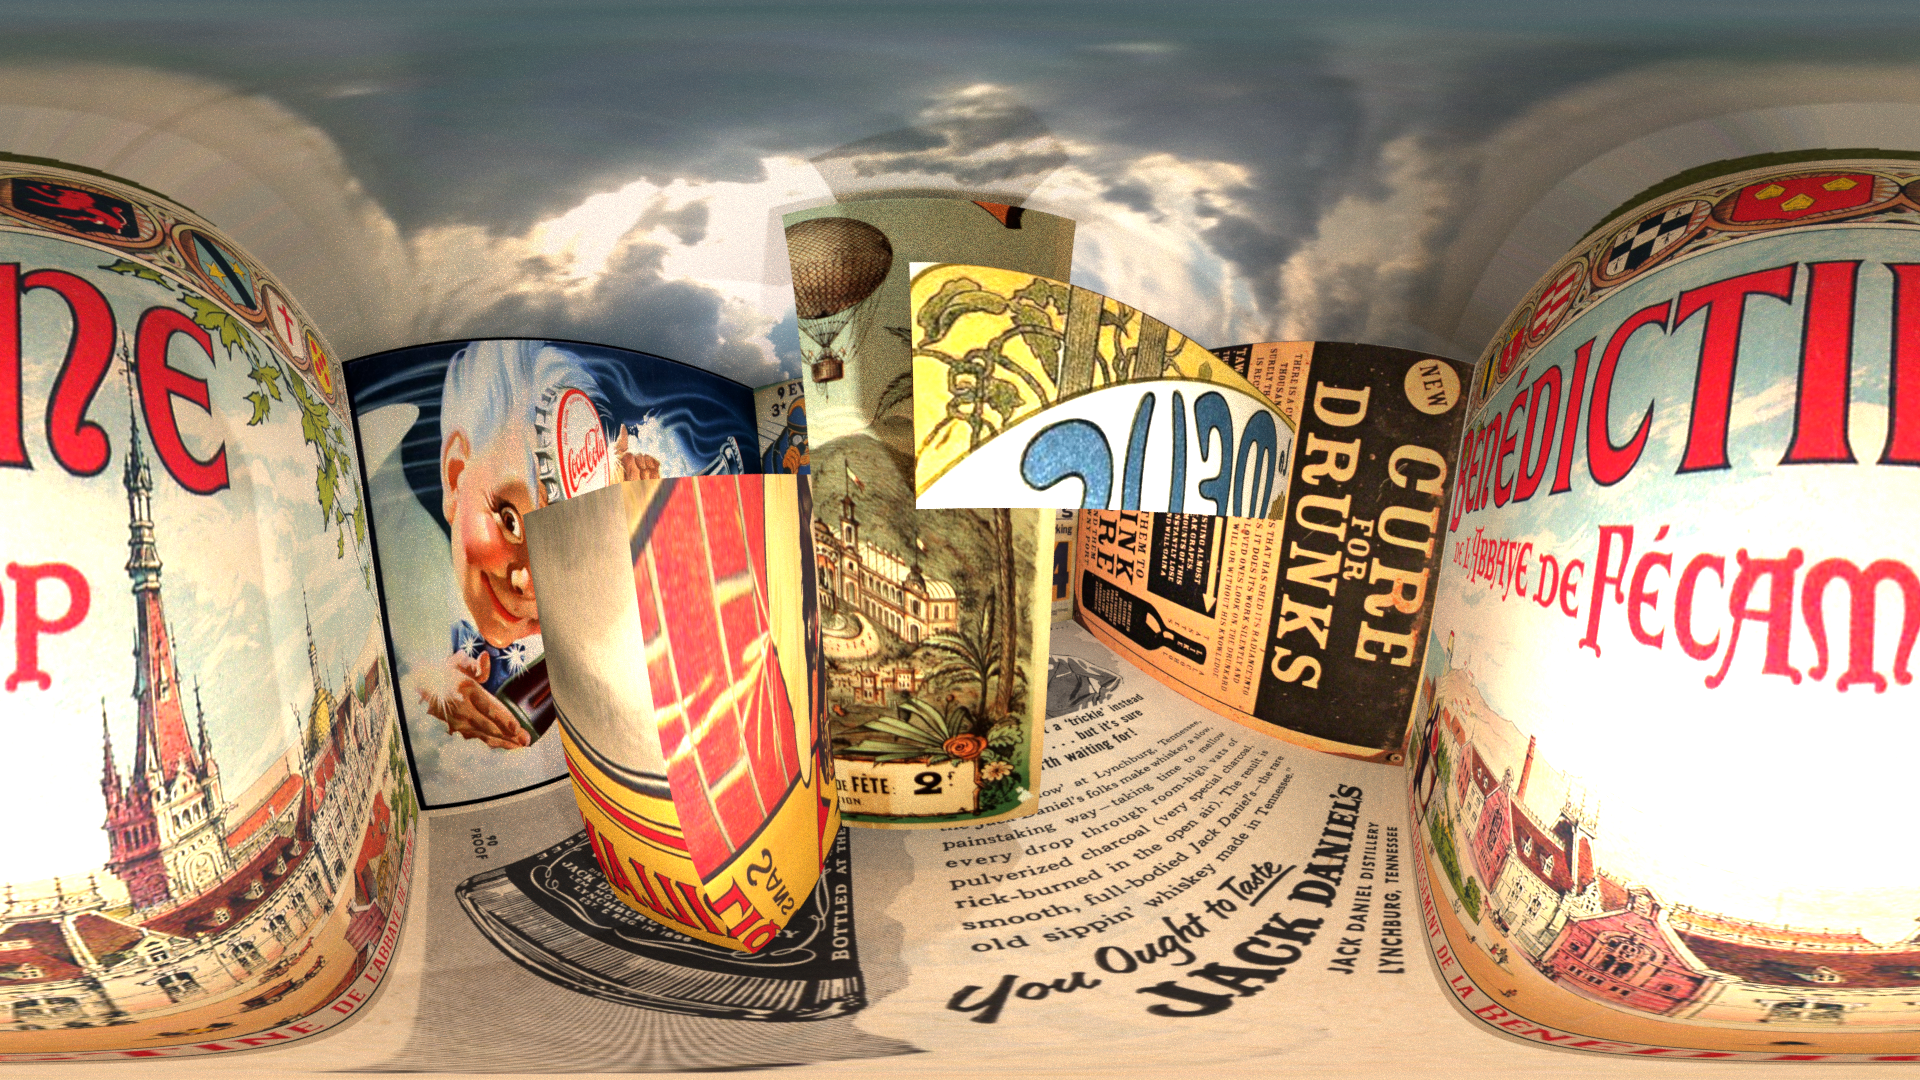
\includegraphics[width=\textwidth]{img/test6_5}
	\end{subfigure}
	%
	\caption{The first computer-generated environment we use in our test and
	an example equirectangular image from this scene.}
    \label{fig:test6}
\end{figure}
%

In the second synthetic scene we recreated a town square sourrounded by
a covered walk (loggia). The roof of the walk is sorrected by columns on the inner
side, the one that is oriented toward the square's centre, and by a wall on the
outer side.
Again the environment is contained in a room and every surface is textured.
The camera moves along the walk with a non-uniform speed while pointing toward
the centre of the square. Figure~\ref{fig:test_square} shows some images
for this second environment.
%
\begin{figure}
\centering
	\begin{subfigure}{0.4\textwidth}
		\centering
		\includegraphics[width=\textwidth]{img/square1}
	\end{subfigure}
    %
	\begin{subfigure}{0.4\textwidth}
		\centering
		\includegraphics[width=\textwidth]{img/square2}
	\end{subfigure}
    %
	\begin{subfigure}{0.8\textwidth}
		\centering
		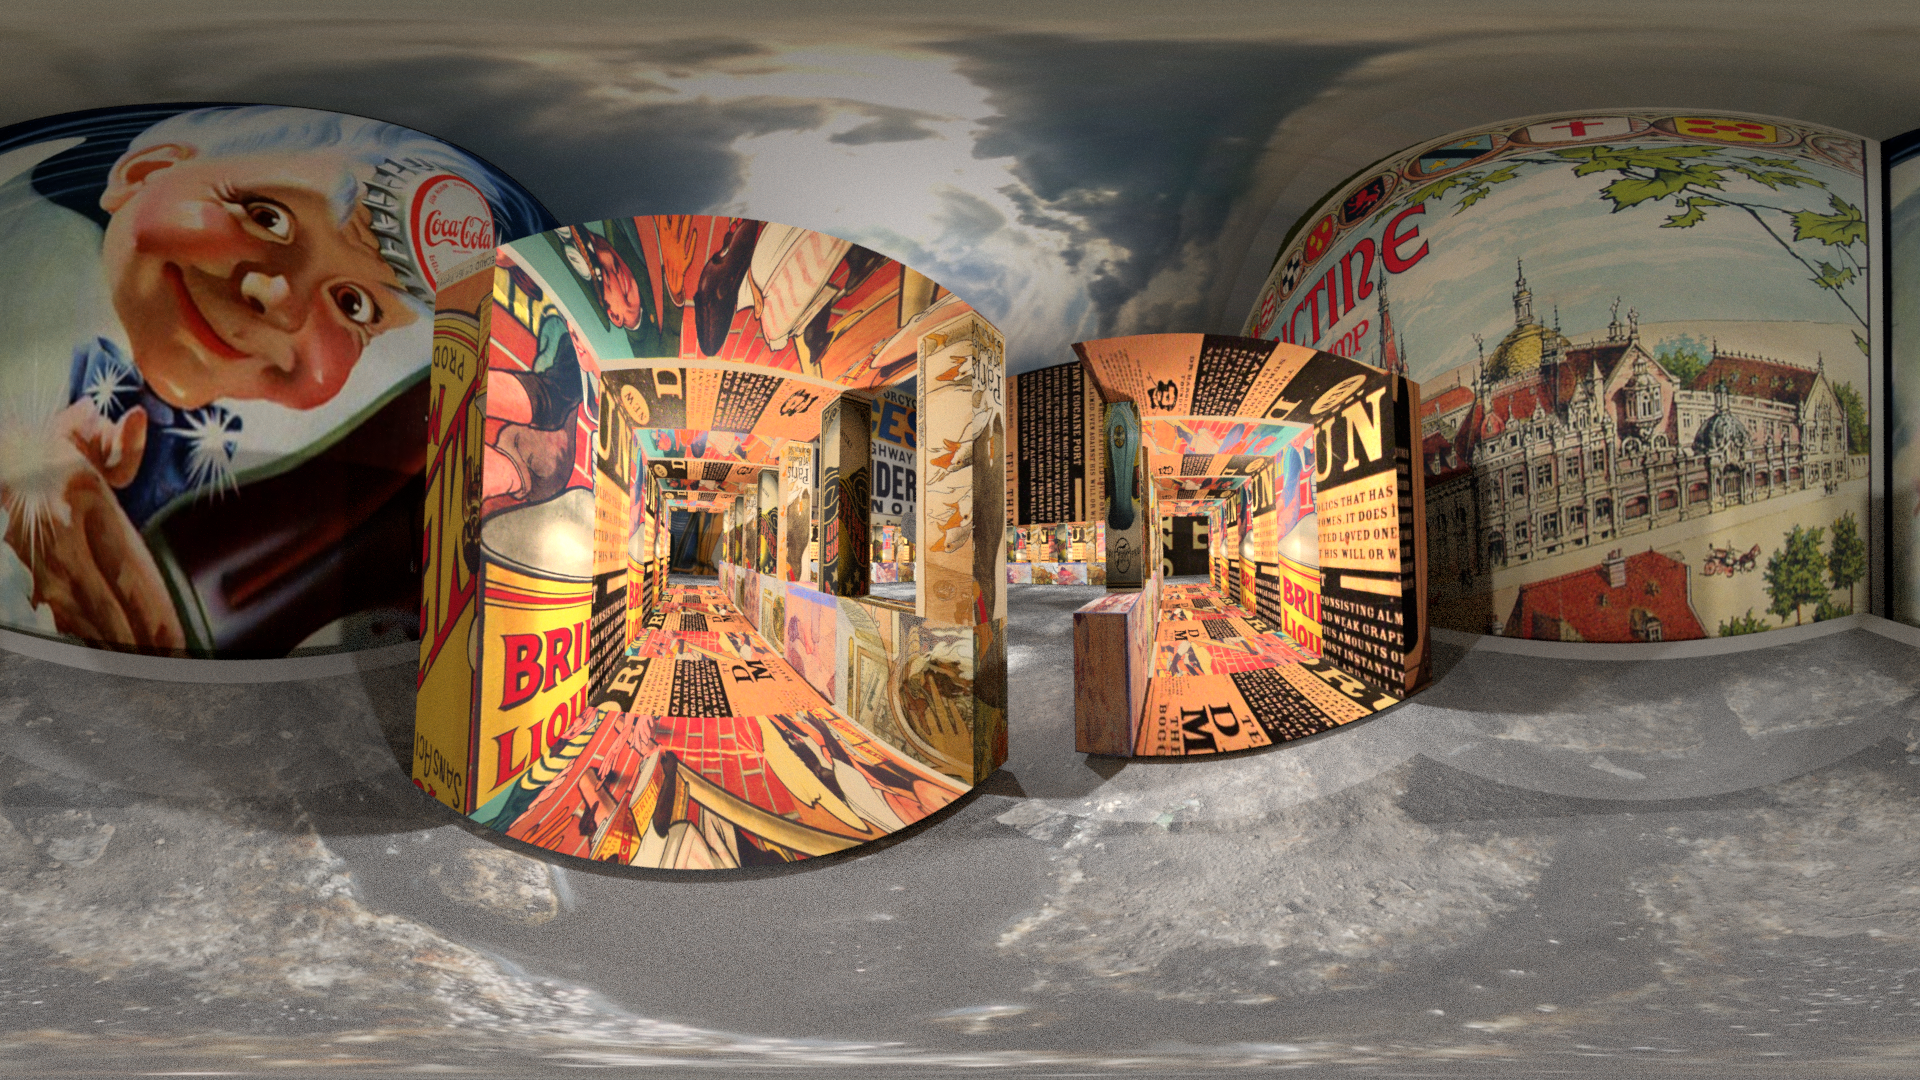
\includegraphics[width=\textwidth]{img/square3}
	\end{subfigure}
    %
	\begin{subfigure}{0.8\textwidth}
		\centering
		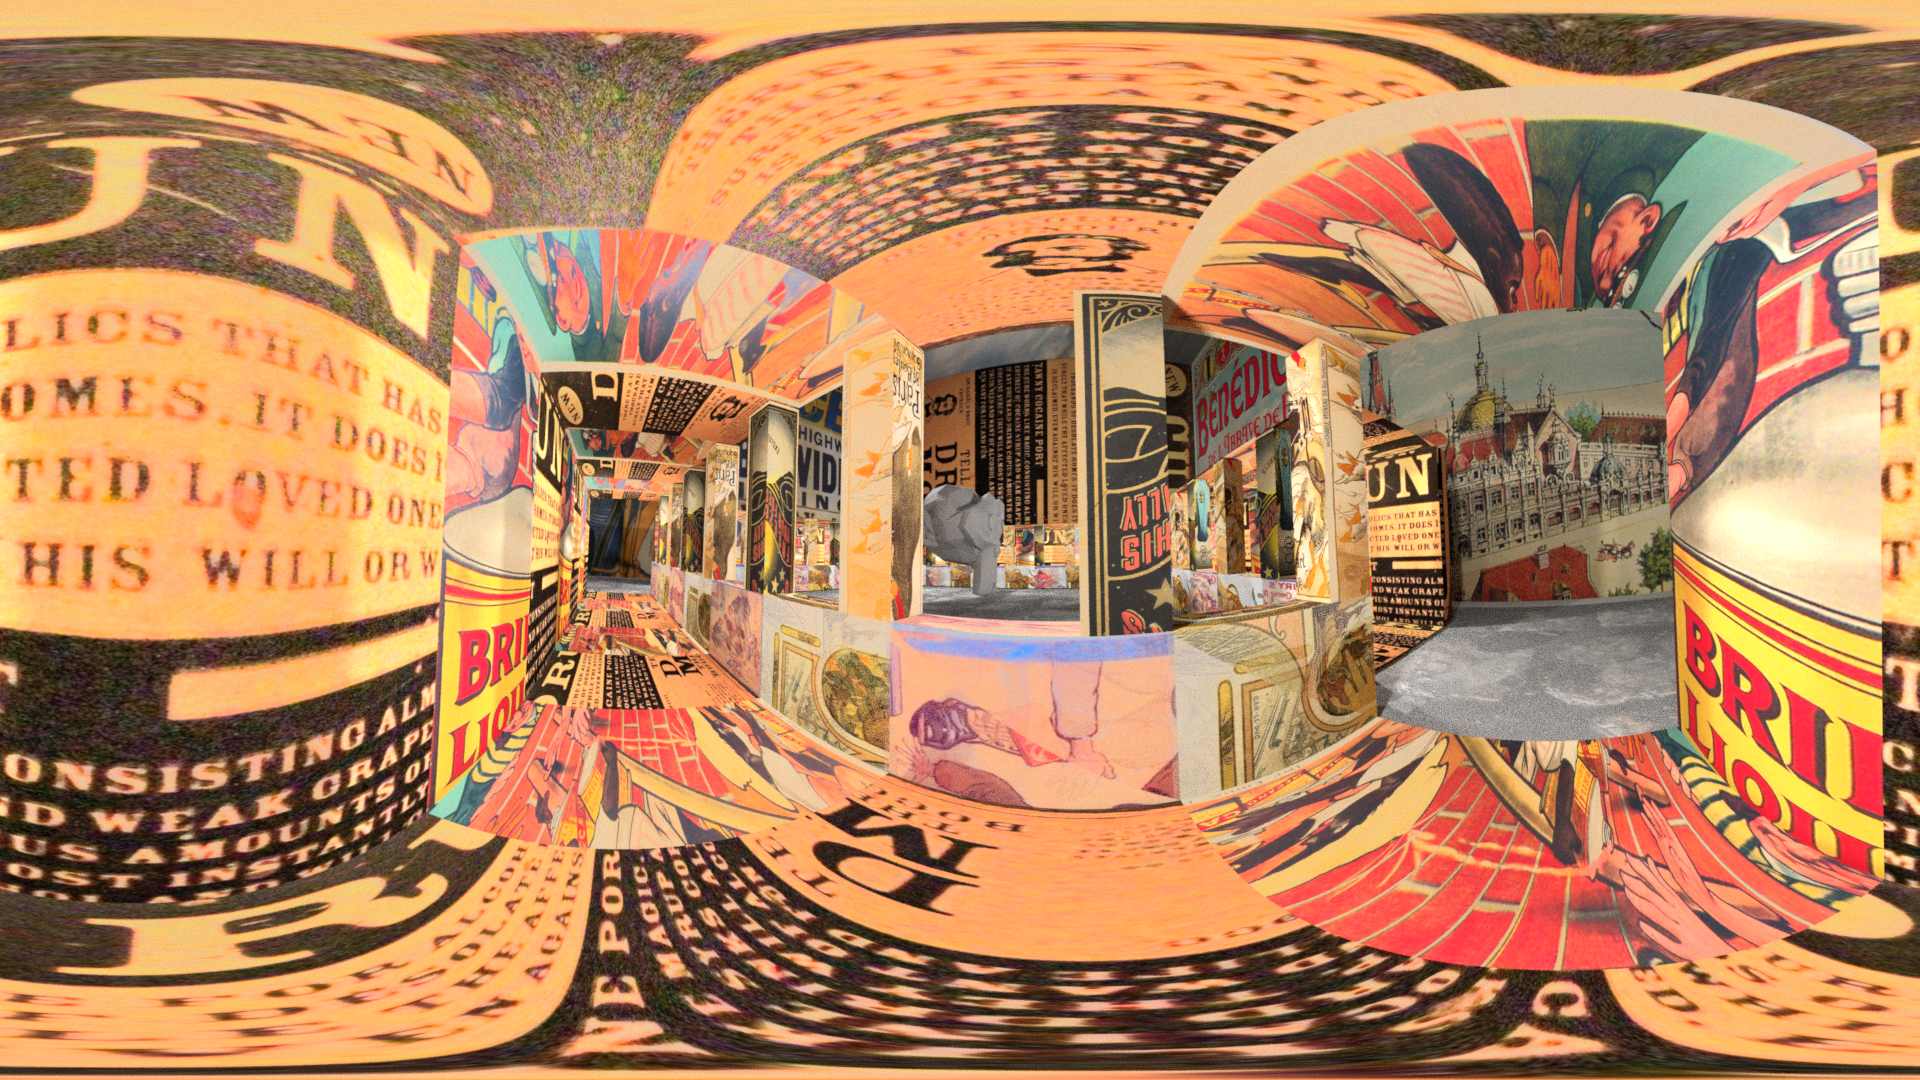
\includegraphics[width=\textwidth]{img/square4}
	\end{subfigure}
	%
	\caption{The computer-generated town square and a couple of example
	equirectangual images from this environment.}
    \label{fig:test_square}
\end{figure}

\section{Real environment}
We test our pipeline with a real video footage too. We do have the ground truth
for the camera poses in the real environment but the quality of the
reconstruction is an indicator of the pipeline performance.
We captured the real sequence with the Ricoh Theta S camera in a town square
sourrounded by a loggia. Again we walked around the square, along the covered
walks, keeping the camera above the user's head thanks to a stick.
The user do not influenced the camera poses estimation since it appears in the
pole region of the image sphere and, as we said in
Section~\ref{sec:pipeline_pose_estimation}, we discard potential matches in
these areas.
We present some pictures of the real environment toghether with some examples
of the equirectangular images of the town square in Figure~\todo{REF}.
%
\missingfigure{aggiungere foto piazza leoni}

%\input{tex/future_work}

\clearpage
\lhead{\emph{\bibname}}
\printbibliography

\end{document}
